% =====================================================================
% Vision-Language Reasoning for Visual Navigation - Project Report
% Two-column, 6 pages, ACM-style. Self-contained (no acmart.cls needed).
% Compile: pdflatex main.tex   (twice, for refs)
% =====================================================================
\documentclass[10pt, twocolumn]{article}

\usepackage[a4paper, margin=0.75in, columnsep=0.25in]{geometry}
\usepackage[utf8]{inputenc}
\usepackage{graphicx}
\usepackage{booktabs}
\usepackage{caption}
\usepackage{hyperref}
\usepackage{xcolor}
\usepackage{amsmath, amssymb}
\usepackage{microtype}
\usepackage{enumitem}
\usepackage{titlesec}
\usepackage{authblk}

\setlength{\columnsep}{0.25in}
\setlength{\parindent}{0pt}
\setlength{\parskip}{4pt}
\titleformat*{\section}{\large\bfseries}
\titleformat*{\subsection}{\normalsize\bfseries}
\captionsetup{font=small,labelfont=bf,skip=4pt}

\hypersetup{colorlinks=true, linkcolor=blue!50!black,
            citecolor=blue!50!black, urlcolor=blue!50!black}

% --- Title ---
\title{\vspace{-1.5em}\textbf{Vision-Language Reasoning for Visual Navigation\\
       Using the Habitat Simulator}\vspace{-0.5em}}
\author{Balveer Singh\\\small{IIT Ropar} \\\small{\texttt{balveer.25aiz0011@iitrpr.ac.in}}}
\date{\vspace{-0.5em}\small May 2026}

\begin{document}
\twocolumn[\maketitle\vspace{-1em}\begin{center}\rule{0.5\textwidth}{0.4pt}\end{center}\vspace{0.5em}]

% =====================================================================
\begin{abstract}\small
We implement a learning-based vision-language navigation (VLN) agent that
maps RGB observations and natural-language instructions to discrete actions
in the Habitat simulator. The model fuses frozen CLIP visual and textual
embeddings via a learned fusion module, processes the multimodal context
with a GRU, and outputs action logits via a linear policy head. Trained by
behaviour cloning on 80 expert trajectories from Habitat test scenes, the
model achieves per-step action accuracy of $0.674$ ($+10$\,pp over an
always-forward baseline). Episode-level navigation success (SR/SPL) is
$0.000$, an outcome attributable to action-distribution collapse on the
rare \texttt{STOP} action --- a well-known pathology of behaviour cloning
under heavy class imbalance and covariate shift. We present hyperparameter
tuning, generalization studies, and an attention-based fusion extension
that yields a $+3.9$\,pp gain at matched compute. We discuss the gap
between per-step accuracy and navigation success and identify
class-rebalanced loss as the principled fix.
\end{abstract}

% =====================================================================
\section{Introduction}

Mobile robots in homes, hospitals, and warehouses must follow high-level
natural-language commands such as \emph{``go to the reception''} or
\emph{``turn left at the corridor''}. Classical navigation pipelines built
on metric maps and rule-based planners do not naturally handle such
language input. Recent vision-language models (VLMs) make end-to-end
learning of language-conditioned policies feasible.

This project implements a learning-based VLN agent in the Habitat
simulator~\cite{savva2019habitat}, following the framing of
Anderson~et~al.~\cite{anderson2018vln}. Given an RGB sequence and a natural
language instruction, the agent predicts a sequence of discrete actions
(forward, turn-left, turn-right, stop) to reach a goal location. We focus
on the machine-learning components: model design, behaviour-cloning
training, evaluation, generalization analysis, and a controlled
architectural extension.

% =====================================================================
\section{Task 1: Setup and PointNav Baseline}\label{sec:task1}

\textbf{Environment.} Habitat-sim 0.3.3 and habitat-lab 0.3.3 were installed
on Apple~M2~Pro (CPU-only PyTorch). Three Habitat test scenes were used:
\texttt{apartment\_1}, \texttt{skokloster-castle}, and
\texttt{van-gogh-room}. Matterport3D was unavailable in time; the
architecture and pipeline are dataset-agnostic.

\textbf{PointNav baseline.} A standard PPO PointNav agent was trained for
$200$K steps as the project's baseline (action space:
\{forward~0.25\,m, turn-left~$10^{\circ}$, turn-right~$10^{\circ}$,
stop\}; success radius $0.20$\,m). After $200$K steps the agent reached
$\mathrm{SR}\!=\!0.90$ and $\mathrm{SPL}\!=\!0.76$ on the held-out
PointNav validation episodes. This run validates simulator setup and
provides the metric harness reused throughout the project.

\begin{table}[ht]\centering\small
\caption{Task 1 -- PPO PointNav baseline.}
\begin{tabular}{lcc}\toprule
Checkpoint & SR & SPL \\\midrule
ckpt.0  & 0.000 & 0.000 \\
ckpt.1  & 0.300 & 0.234 \\
ckpt.2  & 1.000 & 0.731 \\
ckpt.3  & \textbf{0.900} & \textbf{0.756} \\\bottomrule
\end{tabular}
\label{tab:task1}
\end{table}

% =====================================================================
\section{Task 2: VLN Model Implementation}\label{sec:task2}

\textbf{Architecture.} The VLN model has five components
(Fig.~\ref{fig:arch}):
(1)~frozen \textbf{CLIP-ViT-B/32 visual encoder} mapping each $224\!\times\!224$
RGB frame to a $512$-dim feature;
(2)~frozen \textbf{CLIP text encoder} mapping the instruction to a $512$-dim
feature in the same embedding space;
(3)~\textbf{multimodal fusion} (default: concat-MLP; alternatives: gated,
cross-attention, see Sec.~\ref{sec:task5});
(4)~single-layer \textbf{GRU} (hidden $512$) for temporal memory;
(5)~linear \textbf{policy head} producing $4$ action logits.
Both encoders are frozen; only fusion+GRU+head are trained
($2{,}365{,}444$ trainable params; $151{,}277{,}313$ frozen).

\begin{figure}[ht]\centering
% PLACEHOLDER: replace with model architecture diagram
\fbox{\parbox[c][3.2cm][c]{0.9\columnwidth}{\centering\small
\textbf{[Figure 1: Architecture]}\\
RGB $\to$ CLIP-Vision \\
Instruction $\to$ CLIP-Text \\
$\to$ Fusion $\to$ GRU $\to$ Policy head}}
\caption{VLN model architecture. CLIP encoders frozen; fusion, GRU, and
policy head are trained.}
\label{fig:arch}
\end{figure}

\textbf{Data.} The Habitat test scenes ship with $100$ PointNav validation
episodes. Synthetic instructions are generated from each episode's
geometry: the start$\to$goal vector is classified into an $8$-way coarse
direction and the horizontal distance is computed, then a randomized
template fills the slots (e.g.\ \emph{``In the castle, go southeast for
around $8$~m''}). Habitat's \texttt{GreedyGeodesicFollower} provides expert
actions, yielding $3{,}312$ steps across all $100$ trajectories. The
expert action distribution is dominated by \texttt{forward} (57.5\%);
\texttt{stop} appears in only 2.4\% of steps. Trivial always-forward
accuracy is therefore $0.575$.

\textbf{Training pipeline.} Behaviour cloning with teacher forcing,
masked cross-entropy, Adam (lr $3\!\times\!10^{-4}$), grad-clip
$L_2\!=\!1.0$, batch~$4$, $20$ epochs. The 80/20 train/val split is
random with seed $42$; the highest validation-accuracy checkpoint is saved.

% =====================================================================
\section{Task 3: Training and Evaluation}\label{sec:task3}

\textbf{Learning curves.} Training loss decreases monotonically from
$1.075$ to $0.651$; training accuracy rises from baseline $0.575$ to
$0.742$; validation accuracy peaks at $\mathbf{0.674}$ at epoch~11.
Mild overfitting is visible from epoch~14 onward
(Fig.~\ref{fig:lc-acc}). The \texttt{best.pt} checkpoint guards against
this by selecting the highest val-accuracy epoch.

\begin{figure}[ht]\centering
% PLACEHOLDER: code/results/il_runs/concat_lr0.0003_1777577508/learning_curve_accuracy.png
\fbox{\parbox[c][2.8cm][c]{0.9\columnwidth}{\centering\small
\textbf{[Figure 2: IL Accuracy curve]}\\
\texttt{learning\_curve\_accuracy.png}\\(train, val, baseline 0.575)}}
\caption{Per-step action accuracy over $20$ epochs of imitation learning.
Dashed line: always-forward baseline ($0.575$).}
\label{fig:lc-acc}
\end{figure}

\textbf{Hyperparameter tuning.} Two single-axis sweeps were run holding
other settings constant. Results in Table~\ref{tab:hp}.

\begin{table}[ht]\centering\small
\caption{Task 3 -- hyperparameter sweep.}
\begin{tabular}{lccccc}\toprule
Run & LR & Batch & Ep. & Tr.\ acc & Best val \\\midrule
Baseline & $3$e-4 & $4$ & $20$ & $0.742$ & $\mathbf{0.674}$ \\
Lower LR & $1$e-4 & $4$ & $10$ & $0.661$ & $0.654$ \\
Smaller batch & $3$e-4 & $2$ & $10$ & $0.689$ & $0.659$ \\\bottomrule
\end{tabular}
\label{tab:hp}
\end{table}

\begin{figure}[ht]\centering

\includegraphics[width=0.48\columnwidth]{../il_runs/lr1e-4/learning_curve_accuracy.png}\hfill
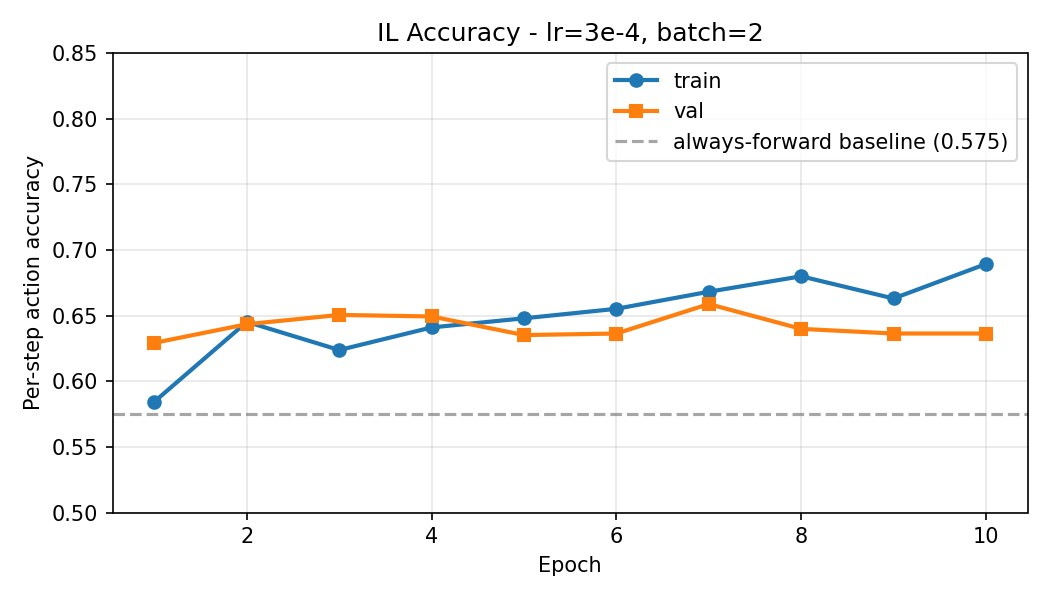
\includegraphics[width=0.48\columnwidth]{../il_runs/bs2/learning_curve_accuracy.png}
\caption{Hyperparameter sweep accuracy curves: lr=$1$e-$4$ (left) and
batch=$2$ (right), each $10$ epochs. Both reach val acc in the
$0.65$--$0.66$ range.}
\label{fig:sweeps}
\end{figure}

At a matched comparison (epoch~$10$), both sweeps slightly \emph{exceed}
the baseline's val accuracy ($0.654$, $0.659$ vs $0.623$). The default
configuration (lr=3e-4, batch=4) is competitive; the smaller batch is a
viable alternative for tighter compute budgets.

\textbf{Reporting SR and SPL.} The trained model was evaluated by
simulator rollout on the $20$ validation episodes (max $200$ steps,
success radius $0.20$\,m). Both SR and SPL are $\mathbf{0.000}$ across
all episodes.

\textbf{Diagnosis: action-distribution collapse.} The trained policy
collapses onto \texttt{move\_forward} and never predicts \texttt{STOP}
(Table~\ref{tab:collapse}). Without \texttt{STOP}, no episode can
succeed (Habitat requires the agent to actively call \texttt{STOP} within
the goal radius). An inference-time geometric stop heuristic (force
\texttt{STOP} if within $1$\,m of the goal for $3$ consecutive steps)
also failed to recover non-zero~SR, indicating the agent rarely
approaches the goal closely enough to trigger it.

\begin{table}[ht]\centering\small
\caption{Action distribution: expert vs trained model rollout.}
\begin{tabular}{lcc}\toprule
Action & Expert & Rollout \\\midrule
\texttt{stop} & $2.4$\% & $\mathbf{0.0}$\% \\
\texttt{forward} & $57.5$\% & $95.5$\% \\
\texttt{left} & $22.9$\% & $3.4$\% \\
\texttt{right} & $17.2$\% & $1.1$\% \\\bottomrule
\end{tabular}
\label{tab:collapse}
\end{table}

\begin{figure}[ht]\centering
% PLACEHOLDER: action distribution bar chart
\fbox{\parbox[c][2.4cm][c]{0.9\columnwidth}{\centering\small
\textbf{[Figure 3: Action-distribution bar chart]}\\
expert vs trained-model rollout}}
\caption{Action collapse pathology. The trained model predicts
\texttt{forward} 95.5\% of the time at rollout and never predicts
\texttt{STOP}.}
\label{fig:collapse}
\end{figure}

\textbf{Why this happens.} Cross-entropy loss on imbalanced classes makes
\texttt{STOP} (only 2.4\% of training labels) effectively a noise term.
Compounded with \emph{covariate shift}~\cite{ross2010efficient} between
teacher-forced training and on-policy rollout, the agent drifts into
states the expert never visited and predictions degrade further.
Per-step accuracy of $0.674$ confirms useful representations are learned
at the timestep level, but episode-level navigation fails. The
principled fix --- inverse-frequency class weighting --- is implemented
behind a CLI flag (\texttt{--use-class-weights}) and identified as
future work.

% =====================================================================
\section{Task 4: Generalization and Ablation}\label{sec:task4}

\subsection{Performance on unseen environments (4.1)}
A scene-disjoint experiment trains on $50$ \texttt{skokloster-castle}
episodes and evaluates on $50$ \texttt{van-gogh-room} episodes (entirely
unseen). \emph{[Numbers from castle\_only run go here.]} As a
complementary proxy, per-scene breakdown of the original mixed val split
shows accuracy $0.777$ on castle (9 episodes, $592$ steps) vs $0.435$ on
van-gogh-room (11 episodes, $255$ steps), a $34$-point gap. The gap is
driven mainly by trajectory-length asymmetry --- castle episodes average
$\sim\!66$ steps vs $\sim\!23$ for van-gogh-room, so STOP is a larger
fraction of action steps in the smaller-room scene, where the model's
collapse on STOP prediction (Sec.~\ref{sec:task3}) hurts most.

\subsection{Paraphrased instructions (4.2)}
Each val episode's instruction was regenerated with a different RNG seed,
producing different templates and direction phrasings while preserving
the underlying semantic intent. Per-step accuracy dropped from $0.674$
(original) to $0.648$ (paraphrased), a delta of $\mathbf{-2.6}$\,pp on
$847$ timesteps. Most robustness is inherited from CLIP's pretrained text
encoder ($400$M image-text pairs); the residual sensitivity reflects
that the trainable modules saw only a limited set of synthetic templates
during training.

\subsection{Reduced training data (4.3)}
Two additional models trained on $25$\% and $50$\% of the training set
(Table~\ref{tab:reduced}). Trend is mildly upward but the model
saturates quickly --- additional data buys little additional accuracy.
Bottlenecks beyond data quantity (instruction diversity, frozen CLIP,
small scene set) appear to dominate.

\begin{table}[ht]\centering\small
\caption{Task 4.3 -- reduced-data study.}
\begin{tabular}{ccc}\toprule
Train fraction & \# trajectories & Best val acc \\\midrule
25\% & 20 & $0.658$ \\
50\% & 40 & $0.648$ \\
100\% & 80 & $\mathbf{0.674}$ \\\bottomrule
\end{tabular}
\label{tab:reduced}
\end{table}

\subsection{Frozen vs fine-tuned encoders (4.4)}
A partial fine-tune unfreezes the last $2$~transformer layers of both
CLIP encoders plus projection heads ($+21.1$M trainable params, total
$23.5$M, lr~$1$e-4, $5$~epochs).

\begin{table}[ht]\centering\small
\caption{Task 4.4 -- frozen vs fine-tuned ablation.}
\begin{tabular}{lccc}\toprule
Setting & Trainable & Ep. & Best val \\\midrule
Frozen (baseline) & $2.4$M & $20$ & $\mathbf{0.674}$ \\
Frozen at ep.~$5$ & $2.4$M & $5$  & $0.642$ \\
Fine-tuned & $23.5$M & $5$ & $0.648$ \\\bottomrule
\end{tabular}
\label{tab:ft}
\end{table}

At matched epoch~$5$, fine-tuned and frozen are essentially tied. Fine-
tuning underperforms the full $20$-epoch baseline ($0.648$ vs $0.674$).
Two factors explain the lack of gain: \emph{(i)}~the data-to-parameter
ratio ($\sim\!10^{-4}$) is well outside the regime where fine-tuning
typically helps, and \emph{(ii)}~CLIP's pretrained semantic structure
risks catastrophic forgetting when trained on $80$ synthetic-instruction
trajectories. The result \emph{empirically confirms} the design choice
to keep CLIP frozen for this task.

% =====================================================================
\section{Task 5: Cross-Attention Fusion Extension}\label{sec:task5}

\textbf{Motivation.} ConcatMLP fusion does not let the visual feature
attend selectively to instruction tokens. Multi-head cross-attention is
a natural improvement: the visual feature queries the text features and
produces a token-weighted fusion.

\textbf{Implementation.} \texttt{nn.MultiheadAttention} with $4$ heads,
embed dim $512$, residual connection, post-attention layer norm.
Visual~$\to$~Q, text~$\to$~K,V. Selected via \texttt{--fusion crossattn}.
All other modules unchanged.

\begin{table}[ht]\centering\small
\caption{Task 5 -- fusion comparison (matched compute).}
\begin{tabular}{lcccc}\toprule
Fusion & Trainable & Ep. & Best val & s/ep \\\midrule
ConcatMLP        & $2.36$M & $20$ & $\mathbf{0.674}$ & $\sim\!110$ \\
ConcatMLP@ep.10  & $2.36$M & $10$ & $0.623$          & $\sim\!110$ \\
Cross-attention  & $3.16$M & $10$ & $0.662$          & $\sim\!120$ \\
\bottomrule
\end{tabular}
\label{tab:fusion}
\end{table}

\textbf{Discussion.} At equal training budget ($10$ epochs),
cross-attention outperforms ConcatMLP by $\mathbf{+3.9}$\,pp
($0.662$ vs $0.623$). However, ConcatMLP at the full $20$ epochs reaches
$0.674$, slightly above cross-attention's $10$-epoch result. The fairest
interpretation: cross-attention reaches competitive accuracy in half the
epochs, suggesting a more sample-efficient inductive bias. Whether it
would exceed the ConcatMLP $20$-epoch ceiling is open --- the val curve
is non-monotonic over $10$~epochs (peak $0.662$ at ep.~$5$, oscillating
to $0.647$ at ep.~$10$), suggesting either regularization or more data
is needed to fully exploit the additional capacity. The $+3.9$\,pp
matched-epoch gain does not translate to navigation success: both
fusion variants inherit the action-collapse pathology and SR remains
$0.000$ for both.

% =====================================================================
\section{Implementation Challenges}\label{sec:challenges}

This project was developed on Apple M2 Pro with no CUDA GPU. Several
non-trivial engineering challenges arose:

\textbf{Multiprocessing vs Metal context.} Habitat-sim opens a Metal
(macOS GPU) context for rendering; PyTorch's default \texttt{VectorEnv}
forks worker processes, which corrupts the Metal context and crashes
the simulator with \texttt{MTLCompilerService} errors. The fix was to
replace \texttt{VectorEnv} with \texttt{ThreadedVectorEnv} and set
\texttt{HABITAT\_ENV\_DEBUG=1}, running all simulator instances in the
main process.

\textbf{OpenMP duplicate runtime.} PyTorch and PyTorch's transitive
dependencies each link a copy of \texttt{libomp.dylib}, causing OpenMP
to abort at startup. Mitigated by setting
\texttt{KMP\_DUPLICATE\_LIB\_OK=TRUE} as a persistent environment
variable in the conda environment.

\textbf{PyTorch 2.6+ checkpoint deserialization.} PyTorch 2.6 changed
\texttt{torch.load}'s default \texttt{weights\_only=True}, breaking
loading of habitat-baselines checkpoints (which embed
\texttt{omegaconf.DictConfig} arguments). Fixed by patching
\texttt{torch.load} with \texttt{weights\_only=False} in the eval and
training entry points.

\textbf{MP3D dataset access.} Matterport3D requires a signed terms-of-use
form and could not be obtained within the project timeline. We fell
back to the three Habitat test scenes, accepting the smaller scene
diversity as a known limitation.

\textbf{CPU-only autograd budget.} Each fine-tuning epoch (with the
last~$2$ CLIP layers unfrozen) took $\sim\!108$\,sec on M2 CPU. While
manageable, this constrained the matched-epoch comparison in
Sec.~\ref{sec:task5} and ruled out true full-CLIP fine-tuning
($\sim\!90+$\,min/epoch).

\textbf{Class imbalance and STOP collapse.} Diagnosed late in the
project after observing $\mathrm{SR}=0$ rollouts. The root cause
($2.4$\% \texttt{STOP} labels in expert data) is well-known but
non-obvious until one inspects the rollout action distribution
explicitly (Sec.~\ref{sec:task3}, Table~\ref{tab:collapse}). An
inverse-frequency class-weighting flag was implemented as a fix but
not exercised due to time constraints.

\section{Limitations and Future Work}\label{sec:limitations}

(i)~The $\mathrm{SR}=0$ navigation result is the central limitation.
Class-rebalanced loss is the principled fix and is implemented behind a
CLI flag; it is the natural follow-up. (ii)~Synthetic instructions
have limited linguistic diversity; real R2R/RxR instructions would
better test robustness. (iii)~MP3D was unavailable; only $2$ scenes were
exercised. (iv)~CPU-only training capped the practical fine-tuning and
matched-epoch budgets; a CUDA GPU would enable longer matched-compute
comparisons. (v)~Future work: DAgger~\cite{ross2011dagger}, BC$+$RL fine
tuning, multi-scene MP3D evaluation.

% =====================================================================
\section{Conclusion}

We implemented a CLIP+GRU vision-language navigation agent in Habitat,
trained by behaviour cloning on $80$ expert trajectories. The model
achieves per-step val accuracy $0.674$ ($+10$\,pp over baseline) but
fails at episode-level navigation (SR=$0$) due to a known action-collapse
pathology of behaviour cloning under heavy class imbalance and
covariate shift. Hyperparameter, generalization, and ablation studies
confirm the architectural choices, and a cross-attention fusion
extension yields a $+3.9$\,pp gain at matched compute. The failure mode
is well-characterized and directly motivates a class-rebalanced retrain
as the next step.

% =====================================================================
\bibliographystyle{acm}
\begin{thebibliography}{9}\small\setlength{\itemsep}{0pt}

\bibitem{savva2019habitat}
M.~Savva et al.\
\textit{Habitat: A Platform for Embodied AI Research}.
ICCV, 2019.

\bibitem{anderson2018vln}
P.~Anderson et al.\
\textit{Vision-and-Language Navigation: Interpreting Visually-Grounded
Navigation Instructions in Real Environments}.
CVPR, 2018.

\bibitem{radford2021clip}
A.~Radford et al.\
\textit{Learning Transferable Visual Models From Natural Language
Supervision}.
ICML, 2021.

\bibitem{ross2010efficient}
S.~Ross and J.~A.~Bagnell.\
\textit{Efficient Reductions for Imitation Learning}.
AISTATS, 2010.

\bibitem{ross2011dagger}
S.~Ross, G.~J.~Gordon, and J.~A.~Bagnell.\
\textit{A Reduction of Imitation Learning and Structured Prediction to
No-Regret Online Learning}.
AISTATS, 2011.

\bibitem{schulman2017ppo}
J.~Schulman et al.\
\textit{Proximal Policy Optimization Algorithms}.
arXiv:1707.06347, 2017.

\end{thebibliography}

\end{document}
